%Cosas Pendientes de Álvaro Rodríguez García

%%%%%%%%%%
% Día 28/2
%%%%%%%%%%

% Después del primer cacho de imágenes directas

Ahora que hemos visto que el caso interesante es que $f$ sea sobreyectiva, consideramos el siguiente diagrama:
\[\xymatrix{
(\X,\T) \ar[r]^{f} \ar[d]_{p} &
(\mc{Y}, f\T) \\
\X/\mathord{\sim}  \ar[ru]_{\bar{f}}
}\]
donde la relación de equivalencia verifica $x\sim y\iff f(x)=f(y)$. Aquí, $p$ es simplemente la aplicación que manda $x\in\X$ a su clase de equivalencia, y consideramos $\bar{f}$ de forma que verifique que $f=\bar{f}\circ p$.

% Esto no lo nombró él en clase pero lo he encontrado por ahí y es cómodo
Decimos que una aplicación $f$ que verifica que si $x\sim y$ entonces $f(x)=f(y)$ respeta la relación de equivalencia $\mathord{\sim}$. Nótese que no se exige la equivalencia, solo la implicación.

Como hemos definido la relación de equivalencia como la que verifica $x\sim y\iff f(x)=f(y)$, tenemos que $\bar{f}$ es una biyección. Además, se puede comprobar que si existe $\bar{f}$ tal que $f=\bar{f}\circ p$, entonces $f$ respeta la relación de equivalencia $\mathord{\sim}$.

Ahora, vamos a definir la topología cociente para $\X/\mathord{\sim}$. Buscamos una topología que verifique que la aplicación $p$ es continua y que existe una aplicación continua $\bar{f}$ que respete la relación de equivalencia $\mathord{\sim}$ y que verifique que $f=\bar{f}\circ p$.

\begin{defi}[Topología cociente]
Definimos la \tbitop[$\T/\mathord{\sim}$]{cociente} en las condiciones anteriores como:
\[\T/\mathord{\sim} = \{V\midc p^{-1}(V)\in\T\}\]
es decir, la topología cociente es la topología imagen por $p$.
\end{defi}

Está claro que se verifican nuestros requisitos. Por un lado, $p$ es trivialmente continua (pues la topología imagen por $p$ es precisamente la que verifica esto). Por otro lado, por ser una topología imagen se verifica directamente la continuidad de $\bar{f}$.

\begin{prop}
	En las condiciones de la construcción (cuando la relación $\sim$ está definida como $x\sim y\iff f(x)=f(y)$), $\bar{f}$ es homeomorfismo.
	
	\begin{proof}
		Ya hemos visto que $\bar{f}$ es biyectivo cuando la relación de equivalencia verifica $x\sim y\iff f(x)=f(y)$; y que es continuo en el sentido en el que lo hemos definido. Para ver la continuidad en el otro sentido, basta con ver que $\bar{f}$ es abierta.
		
		En efecto, $U\in \X/\mathord{\sim}$ abierto $\iff p^{-1}(U)$ es abierto en $\X$. Pero tenemos que $p^{-1}(U)=f^{-1}(f(S))$, porque:
		\[x\in p^{-1}(U)\iff p(x)\in S\stackrel{\bar{f}\text{ biy.}}{\iff}\bar{f}(p(x))\in \bar{f}(U)\iff f(x)\in\bar{f}(U)\iff x\in f^{-1}(\bar{f}(U))\]
		
		Entonces, como $f(\T)$ es la topología en $\mc{Y}$, $f^{-1}(f(U))$ es abierto en $\X\iff \bar{f}(U)$ es abierto en $\mc{Y}$, pero ya hemos visto que $f^{-1}(f(U))$ es abierto, porque es $p^{-1}(U)$.
	\end{proof}
\end{prop}

Por otro lado, está claro que todos los abiertos de $\T/\mathord{\sim}$ son imágenes por $p$ de abiertos de $\T$ (pero no todas las imágenes de abiertos tienen que estar necesariamente en $\T$). Entonces, definimos:

\begin{defi}[Conjunto saturado]
En las condiciones anteriores, decimos que $W\in\T$ es \tbi[conjunto!saturado]{saturado} si $W=p^{-1}(p(W))$. Es equivalente decir que $[x]\cap W\neq\emptyset\implies [x]\subset W$, o que $x\in W,y\sim x\implies y\in W$.
\end{defi}

Gracias a esta definición, podemos reescribir la topología cociente como:
\[\T/\mathord{\sim} = \{p(W)\midc W\in\T\text{, } W\text{ saturado}\}\]

Además, vamos a dar un nombre a las funciones que envían $X$ en un espacio homeomorfo a un cociente:

\begin{defi}[Identificación]
	Una \tbi{identificación} es una aplicación $f:(X,\T)\to (\mc{Y},\T')$ sobreyectiva que verifica que $\T'$ es la topología imagen por $f$ $f(\T)$.
\end{defi}

La aplicación $f$ con la que hemos estado trabajando es, entonces, una identificación. El hecho de que la topología de $\mc{Y}$ sea la imagen significa que una identificación es continua.

Las identificaciones se llaman a veces en la literatura aplicaciones cociente\index[general]{aplicación!cociente}. Esto está ligado con su utilidad: las identificaciones son aquellas que inducen una relación de equivalencia $\sim$ de forma que podemos desarrollar toda la construcción anterior. De esta forma, nos ``regalan'' un espacio homeomorfo a $\mc{Y}$ que a menudo es más simple y más fácil de entender que él. Este propósito quedará más claro en los ejemplos posteriores.

Para comprobar si una aplicación es una identificación, podemos usar la siguiente proposición:

\begin{prop}[Condiciones suficientes de identificación]
Sea $f:\X\to\mc{Y}$ una aplicación. Si se verifica alguna de las siguientes condiciones, $f$ es una identificación:
\begin{enumerate}
\item $f$ es una aplicación continua abierta.
\item $f$ es una aplicación continua cerrada.
\end{enumerate}
\end{prop}

Nótese que puede haber identificaciones que no verifiquen ninguna de las condiciones anteriores. Además, como no se exige que las identificaciones sean biyectivas, las dos condiciones anteriores no son equivalentes.

Toda esta construcción abstracta debe servirnos para formalizar todo el concepto de cociente de un espacio. Esta es quizá la idea más importante que se va a ver en toda la asignatura, y es excepcionalmente útil para construir una gigantesca variedad de homeomorfismos y encontrar objetos simples homeomorfos a otros mucho más complejos.



\begin{exa}[Circunferencia unidad]
	Definimos la aplicación:
	\[\begin{split}
	\R&\to\esfera^1 \\
	t&\mapsto e^{2\pi it}=(\cos 2\pi t,\sen 2\pi t)
	\end{split}\]
	y consideramos la relación de equivalencia $s\sim t\iff e^{2\pi is}=e^{2\pi it}\iff s-t\in\Z$. Vamos a ver que la circunferencia unidad $\esfera^1$ es homeomorfa a $\R/\mathord{\sim}$.
	
	Nos queda, pues, el siguiente esquema:
	\[\xymatrix{
		\R \ar[r] \ar[d] &
		\esfera^1 \\
		\R/\mathord{\sim}  \ar@{<->}[ru]
	}\]
	y está claro que la aplicación que manda $f$ a $\esfera^1$ es una identificación, pues es sobreyectiva, continua y homeomorfismo local, luego es abierta.
	
	Ahora, nótese que considerando $[0,1]\subset\R$ podemos tomar las restricciones correspondientes con el siguiente esquema:
	\[\xymatrix @C=0.5pc @R=0.5pc @L=-0.2pc {
	    & \R \ar[rr] \ar[dd] & &
		\esfera^1 \\
		[0,1] \ar@{}[ur]^*[@]{\subset} \ar[dr] \\
		& \R/\mathord{\sim}  \ar@{<->}[rruu]
	}\]
	y llegar a otra identificación. Ahora la relación de equivalencia asociada es simplemente aquella en la que $1\sim 0$ y todos los demás puntos son solamente equivalentes a sí mismos.
\end{exa}

Esta posibilidad de encontrar, a veces, un cociente más simple que tiene la misma topología nos motiva a definir:

\begin{defi}[Dominio fundamental]
	En una construcción como la anterior, llamamos \tbi{dominio fundamental} a la región cerrada más pequeña posible con un representante de cada clase de equivalencia. Según la situación, a veces se exigen también otras propiedades como compacidad.
\end{defi}

\begin{exa}
	Ahora, vamos a considerar el toro de revolución que vive en $\R^3$, cuya parametrización es conocida:
	\[\begin{split}
	x&=(a\cos(\theta)+b)\cos(\phi),\\
	y&=(a\cos(\theta)+b)\sin(\phi),\\
	z&=a\sin(\theta).
	\end{split}\]
	
	Como vemos en la imagen, se trata de una figura generada por revolución de una circunferencia en torno a un eje.
	
	\begin{figure}[h!]
		\centering
		
\includegraphics[scale = 0.15]{img/toro}
	\end{figure}

	Vamos a hacer pues una construcción similar a la ya vista para la circunferencia unidad. Nos queda un esquema del siguiente tipo:
	
	\[\xymatrix @C=0.5pc @R=0.5pc @L=-0.2pc {
		& \R^2\ar[rr] \ar[dd] & &
		\toro^2\subset\R^3 \\
		[0,2\pi]^2 \ar@{}[ur]^*[@]{\subset} \ar[dr] \\
		& \R^2/\mathord{\sim}  \ar@{<->}[rruu]
	}\]

	En este caso, la relación de equivalencia está definida como:
	\[(x,y)\sim (x',y')\iff x-x'\in\Z,\;y-y'\in\Z\]
	y como dominio fundamental encontramos el cuadrado $[0,2\pi]^2$. 
	
	A menudo, los dominios fundamentales se representan con esquemas como el siguiente, que representa el toro que acabamos de describir:
	
	% Copiado de https://en.wikipedia.org/wiki/Fundamental_polygon . Querría hacer uno yo pero no ha dado tiempo.
	\begin{figure}[h!]
		\centering
		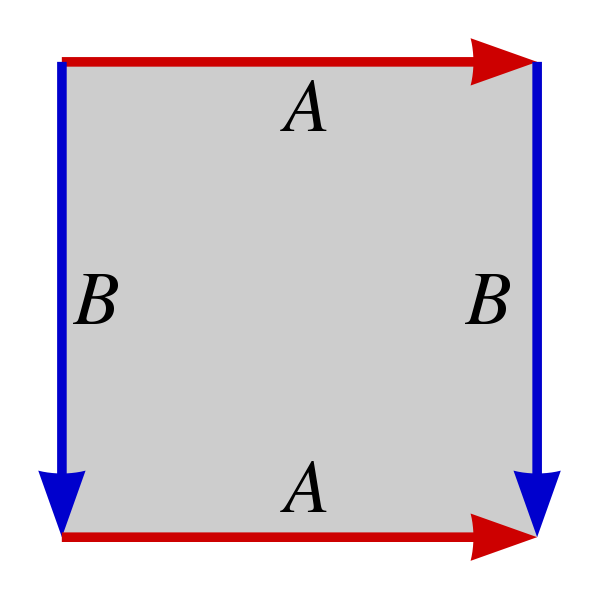
\includegraphics[scale = 0.1]{img/pol_fund_toro}
	\end{figure}

	Estos esquemas se llaman \tbi[polígono fundamental]{polígonos fundamentales}. La forma de entenderlos es que la relación de equivalencia ``pega'' los puntos de $A$ y de $B$ en el sentido que indican las flechas.
\end{exa}

En el siguiente ejemplo, vamos a ver varios homeomorfismos cociente importantes pero sin entrar en tantos detalles como en los ejemplos previos. Para familiarizarnos íntimamente con el espacio cociente, es un buen ejercicio mental tratar de visualizar cómo podemos deformar un objeto del ejemplo siguiente para transformarlo en otro homeomorfo. Al fin y al cabo, la homeomorfia, intuitivamente, es poder deformar sin romper, y los cocientes formalizan la noción de ``pegar'' puntos.

\begin{exa} \
	\begin{enumerate}
		\item La esfera $\esfera^2$ se puede identificar con el disco unidad si la relación de equivalencia es la que hace que todos los puntos del borde estén relacionados entre sí y los demás, solo con sí mismos. De la misma forma, la podemos identificar con dos discos donde la relación de equivalencia ``pega'' los bordes. Por último, una esfera tiene como polígono fundamental:
		
		\begin{figure}[h!]
			\centering
			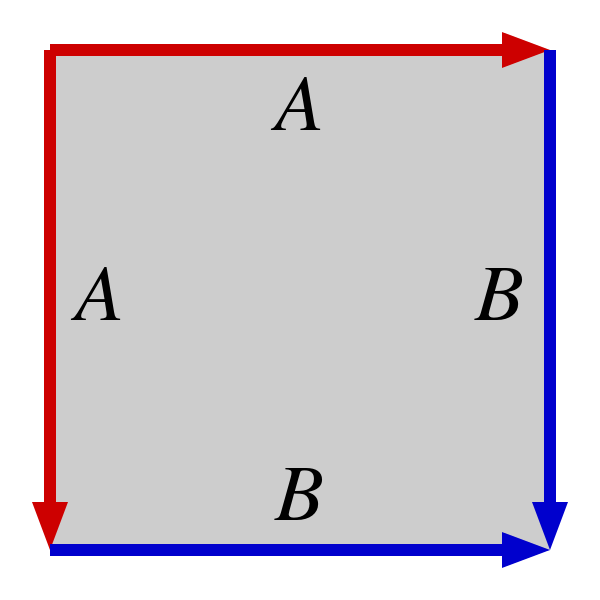
\includegraphics[scale = 0.1]{img/pol_fund_esfera}
		\end{figure}
	
		\item Podemos identificar el plano proyectivo real $\proy^2$ con un disco y una esfera donde la relación de equivalencia ``pega'' los bordes. También podemos identificarlo con una semiesfera en la que cada punto del borde es equivalente a su antípoda, o con una esfera completa en la que dos puntos están relacionados si y solo si son antipodales. Además, el polígono fundamental del plano proyectivo real sería:
		
		\begin{figure}[h!]
			\centering
			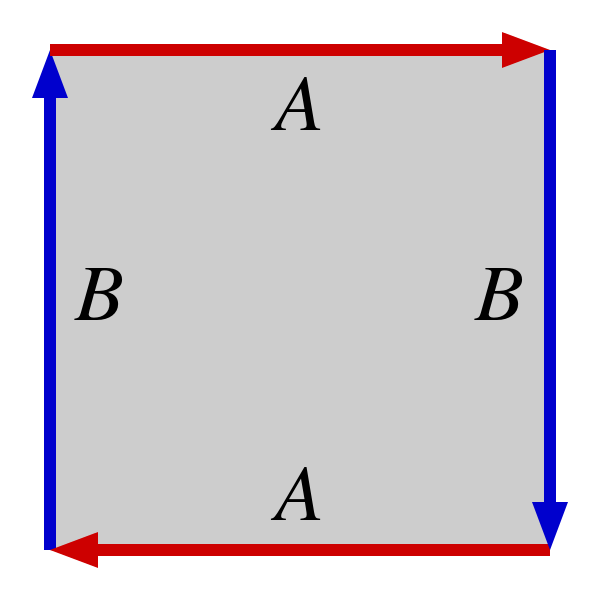
\includegraphics[scale = 0.1]{img/pol_fund_plano_proy}
		\end{figure}
	
		\item Vamos a ver otros dos polígonos fundamentales más. El de la banda de Möbius sería:
		
		\begin{figure}[h!]
			\centering
			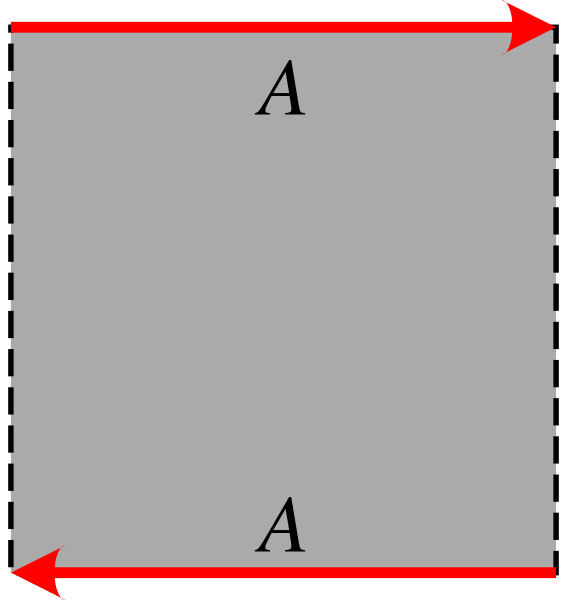
\includegraphics[scale = 0.09]{img/pol_fund_mobius}
		\end{figure}
	
		Nótese que en este caso hay un lado que no se pegaría, que corresponde al borde de la banda de Möbius. 
		
		Por otro lado, el de la botella de Klein sería:
		\begin{figure}[h!]
			\centering
			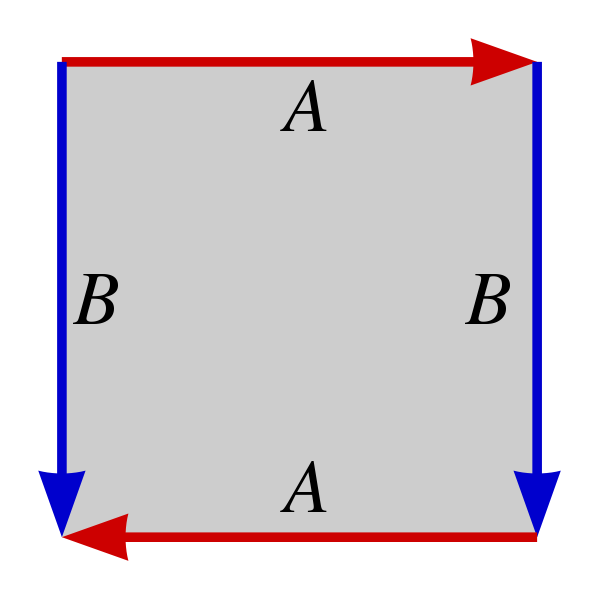
\includegraphics[scale = 0.1]{img/pol_fund_botella_klein}
		\end{figure}
	\end{enumerate}
\end{exa}